\documentclass{deltares_manual_style}
\usepackage{enumitem}
\usepackage{amssymb,amsmath}
\usepackage{xcolor,colortbl,color}
\usepackage{tabularx}
\usepackage{tabulary}
\usepackage{hyperref}
\usepackage{float}
\usepackage{placeins}
%------------------------------------------------------------------------------
\hypersetup
{
    pdfauthor   = {Deltares},
    pdftitle    = {Kratos Geomechanics Application},
    pdfkeywords = {Deltares, User Manual},
    pdfcreator  = {LaTeX hyperref},
    pdfproducer = {ps2pdf}
}
%------------------------------------------------------------------------------
%
\renewcommand\BackgroundPicPart{
    \put(0,0){
        \parbox[b][\paperheight]{\paperwidth}{%
            \vspace{8\baselineskip}
            \hspace{44mm} % 20mm wegens leftmarginskip + 24 mm ~ 1 inch
%           \includegraphics[width=\paperwidth, height=\paperheight, keepaspectratio]{pictures/dsheetpiling-part.png}%
            \vfill
        }
    }
}
% Todo add a ribbon?
%\renewcommand\BackgroundPicChapter{
%    \put(0,0){
%    \parbox[b][\paperheight]{\paperwidth}{%
%        \vspace{4\baselineskip}
%        \hspace{220mm}
%       \includegraphics[width=15mm]{pictures/ribbon.jpg}%
%        \vfill
%        }
%    }
%}

\begin{document}
% TODO insert pdf cover 
% \pagestyle{empty}
%\includepdf[pages=1,offset=72 -70]{pictures/cover_user_manual.pdf} % First and last page
%\cleardoublepage

\title{\textsc{Kratos Geomechanics}}
\subtitle{Finite element model}
\manualtype{Verification Report}
\version{0.1}
\manualtitle

\chapter{Introduction}\label{intro}
This document contains verification examples for the Kratos-Geomechanics application. To achieve this different benchmarks 
are created to test different parts of the Kratos-Geomechanics application. 
 
\chapter{Benchmark 1: Bi-axial shearing test with linear elastic model} \label{chap:bench1}
In this benchmark Bia-axial shearing test conditions are tested in the Kratos-Geomechanics application. In that way, 
this example can be used to verify elastic deformation with a linear elastic model.

\section{Geometry and boundary conditions}
The geometry created in Kratos is a 2-D square specimen ($1\times1m^{2}$). To create the geometry click on the \textit{Create line}
button and enter the points as they are described in \autoref{tab:CoordinatesOfSquareSpeciment}. After creating the square specimen
a surface needs to be created so that the soil elements can be assigned to it. This can be done by clicking the \textit{create NURBS surface} and then the surface of the square specimen created. 
\begin{table*}[h]
	\caption{Coordinates of square specimen}
	\label{tab:CoordinatesOfSquareSpeciment}
	\centering
		\begin{tabular}{|c|c|}
			\hline
			x-coordinate & y-coordinate \\ \hline
			0 & 0 \\ \hline
			0 & 1 \\ \hline
			1 & 1 \\ \hline
			1 & 0 \\ \hline
			0 & 0 \\ \hline
		\end{tabular}
\end{table*}

For the boundary conditions the following constrains are applied to the model:
\begin{itemize}
	\item a \textit{Solid Displacement} is used to fix the bottom boundary in the y direction. By setting the \textit{SOLID DISPLACEMENT Y} to <0.0>.
	\item a \textit{Solid Displacement} is used to fix the bottom left corner in the x and the y direction. By setting
	the \textit{SOLID DISPLACEMENT Y} and the \textit{SOLID DISPLACEMENT X} to <0.0>.
\end{itemize}

The loads applied to the geometry are line load in this case and they are applied to the edges of the geometry. This is done by
selecting the \textit{Loads} menu and inputting the loads that are shown in \autoref{tab:loadinputbench1}.
\begin{table*}[h]
	\caption{Line Load inputs for benchmark 1}
	\label{tab:loadinputbench1}
	\centering
		\begin{tabular}{|c|c|c|c|c|}
			\hline
			Direction  & Assigned Line  & Assigned Line  & Value  & Unit \\
			Setting & Coordinate x & Coordinate y & & \\ \hline
			LINE LOAD X & [0,1] & [1,1] & -1 & N/m \\ \hline
			LINE LOAD X & [0,0] & [1,0] & +1 & N/m \\ \hline
			LINE LOAD Y & [0,0] & [0,1] & -1 & N/m\\ \hline
			LINE LOAD Y & [1,1] & [0,1] & +1 & N/m \\ \hline
		\end{tabular}
\end{table*}

\section{Material}
The material selected for this benchmark is a linear elastic drained soil material. The inputs of this can be seen in
\autoref{fig:material_bm_1} and can be set on the \textit{Elements} menu item.
\begin{figure}[H]
	\centering
		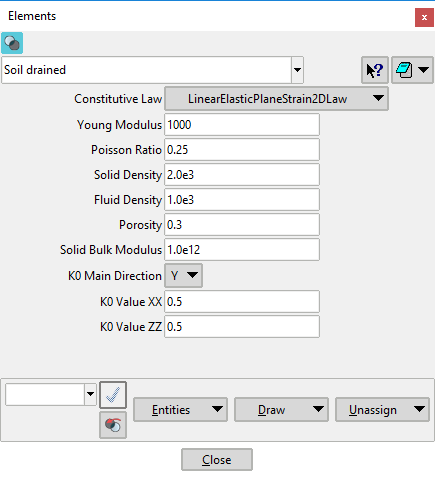
\includegraphics[width=0.5\textwidth]{figures/material_bm_1.png}
	\label{fig:material_bm_1}
	\caption{Material input of benchmark 1}
\end{figure}

\section{Mesh Generation}
The mesh in this case should be generated coarsely. In this case only two elements will be produced. To produce the mesh
click on \textit{Mesh} menu and then from the drop down list select \textit{Generate mesh} and enter for \textit{Enter
size of elements to be generated} <1>.  
\section{Results} 
 The Kratos-Geomechanics application uses as output strain tensor the \textit{Green-Langrange-Strain-Tensor}. The output of the calculation in this case is $\epsilon_{xy} = 1.25\times10^{-3}$ which is half of shear strain $\tau$.
Therefore, the shear strain is $\tau= 2.5\times10^{-3}$.

The analytical solution can be calculated as follows from \autoref{eq:shearmoduluscalc} and \autoref{eq:shearstraincalc}. 
\begin{equation} \label{eq:shearmoduluscalc}
G = \frac{E}{1( 1 + \nu')} = 400 kN/m^{2} 
\end{equation}

\begin{equation}\label{eq:shearstraincalc}
\tau = \frac{\gamma}{G} = 2.5\times10^-{3} for \tau=1 kN/m 
\end{equation}

The comparison of the displacements calculated by Kratos can be compared with the results of the analytical solution in
\autoref{tab:Resultsbm1}.

\begin{table}[H]
	\caption{Results of displacements for benchmark1 }
	\label{tab:Resultsbm1}
	\centering
		\begin{tabular}{|c|c|c|}
			\hline
			Kratos & Benchmark & Error[\%] \\ \hline
			$2.50\times10^{-3}$ & $2.50\times10^{-3}$ & $0.00$ \\ \hline
		\end{tabular}
\end{table}

To run this benchmark run file smoothrigidfootingonelasticsoil.gid.

\chapter{Benchmark 2: Bending of plates} \label{Bench2}
In this benchmark the bending of plate elements with Kratos-Geomechanics will be tested. Two different plate elements of 
unit length are tested. In the first case a point load is applied on the first plate and the second case 
a line load is applied in the second plate. The plates are modeled in 2D geometry thus the material used to model the
plates are beam elements.     
\section{Bending of plate when point load is applied}
\subsection{Geometry}
In this case a line of 1m needs to be created. To create the line click on the \textit{Create line} button and enter the 
points that are part of \autoref{tab:platebend2.1}.
\begin{table*}[h]
	\caption{Coordinates plate element}
	\label{tab:platebend2.1}
	\centering
		\begin{tabular}{|c|c|}
			\hline
			x-coordinate & y-coordinate \\ \hline
			0 & 0 \\ \hline
			0.5 & 0 \\ \hline
			1 & 0 \\ \hline
		\end{tabular}
\end{table*}

The beam is simply-supported so solid displacements are used to model the fixities at the points. For points <0,0> and 
<1,0> a \textit{Solid Displacement} of <0.0> is applied for x and y direction. 

The point load is applied on point <0.5,0> from the menu item \textit{Loads}. By selecting \textit{Point Load} and 
setting \textit{POINT LOAD Y} to <100N> the load can be defined.  
 
\subsection{Material}
The material of the plate element can be defined by selecting the menu item \textit{Elements} and then filling out the 
values of \autoref{fig:beam_bm_2.1}.

\begin{figure}[h]
	\centering
		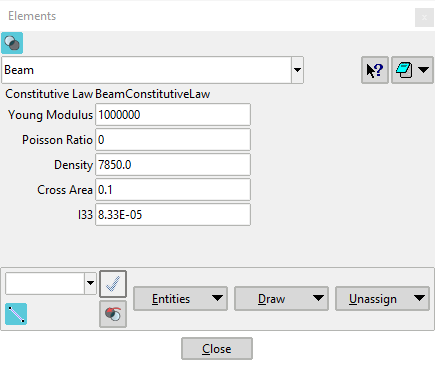
\includegraphics[width=0.50\textwidth]{figures/beam_bm_2_1.png}
	\caption{Beam element of benchmark 2}
	\label{fig:beam_bm_2.1}
\end{figure}

\subsection{Results} 
% ToDo : when issue #7 is done add the part about bending moments and shear stresses.
In this benchmark the result of the maximum deflection is compared with the analytical result. The analytical
calculation of simply supported beam with point load at the center is described in \autoref{eq:disp2.1}. In this case $F = 100kN$ , 
$l = 1m$ and $EI = 83.33 kNm^{2}/m$.

\begin{equation}\label{eq:disp2.1}
u_{max} = \frac{1}{48} \frac{F l^{3}}{EI} = 25.00mm
\end{equation}

After performing the calculation in Kratos-Geomechanics the results are compared with the benchmark in \autoref{tab:Resultsbm2.1} 

\begin{table}[H]
	\caption{Results of deflection for benchmark 2 with the application of point load }
	\label{tab:Resultsbm2.1}
	\centering
		\begin{tabular}{|c|c|c|}
			\hline
			Kratos & Benchmark & Error\\ \hline
			[mm] & [mm] & [\%] \\ \hline  
			$25.01$ & $25.00$ & $0.04$ \\ \hline
		\end{tabular}
\end{table}

\section{Bending of plate when line load is applied}
\subsection{Geometry}
In this case a line of 1m needs to be created. To create the line click on the \textit{Create line} button and enter the 
points that are part of \autoref{tab:platebend2.2}.
\begin{table*}[h]
	\caption{Coordinates plate element}
	\label{tab:platebend2.2}
	\centering
		\begin{tabular}{|c|c|}
			\hline
			x-coordinate & y-coordinate \\ \hline
			0 & 0 \\ \hline
			1 & 0 \\ \hline
		\end{tabular}
\end{table*}

The beam is simply-supported so solid displacements are used to model the fixities at the points. For points <0,0> and 
<1,0> a \textit{Solid Displacement} of <0.0> is applied for x and y direction. 

The line load is applied on the full length of the beam from the menu item \textit{Loads}. By selecting \textit{Line Load} and 
setting \textit{POINT LOAD Y} to <200N/m> the load can be defined.  
 
\subsection{Material}
The material of the plate element can be defined by selecting the menu item \textit{Elements} and then filling out the 
values of \autoref{fig:beam_bm_2.2}.

\begin{figure}[h]
	\centering
		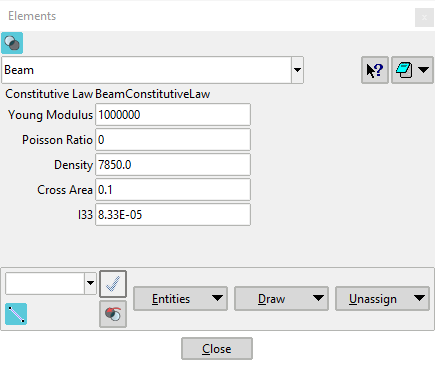
\includegraphics[width=0.50\textwidth]{figures/beam_bm_2_2.png}
	\caption{Beam element of benchmark 2}
	\label{fig:beam_bm_2.2}
\end{figure}

\subsection{Results} 
% ToDo : when issue #7 is done add the part about bending moments and shear stresses.
In this benchmark the result of the maximum deflection is compared with the analytical result. The analytical
calculation of simply supported beam with line load at the center is described in \autoref{eq:disp2.2}. In this case $q = 100kN/m$ , $l = 1m$ and $EI = 83.33 kNm^{2}/m$.

\begin{equation}\label{eq:disp2.2}
u_{max} = \frac{5}{ 384} \frac{q l^{4}}{EI} = 31.25mm
\end{equation}

After performing the calculation in Kratos-Geomechanics the results are compared with the benchmark in \autoref{tab:Resultsbm2.2} 

\begin{table}[H]
	\caption{Results of deflection for benchmark 2 with the application of line load }
	\label{tab:Resultsbm2.2}
	\centering
		\begin{tabular}{|c|c|c|}
			\hline
			Kratos & Benchmark & Error\\ \hline
			[mm] & [mm] & [\%] \\ \hline  
			$31.25$ & $31.25$ & $0.00$ \\ \hline
		\end{tabular}
\end{table}

To run this benchmark run file Kratos\_line\_load.gid and bendingofplatepointload.gid.



\chapter{Benchmark 3: Smooth rigid footing on elastic soil}
In this benchmark a smooth rigid footing is tested on elastic soil with Kratos-Geomechanics. 

\section{Geometry}

A uniform displacement of 0.01 m is applied

The geometry and mesh is shown in \autoref{fig:rigid_footing__geometry_bm_3}

\begin{figure}[h]
	\centering
	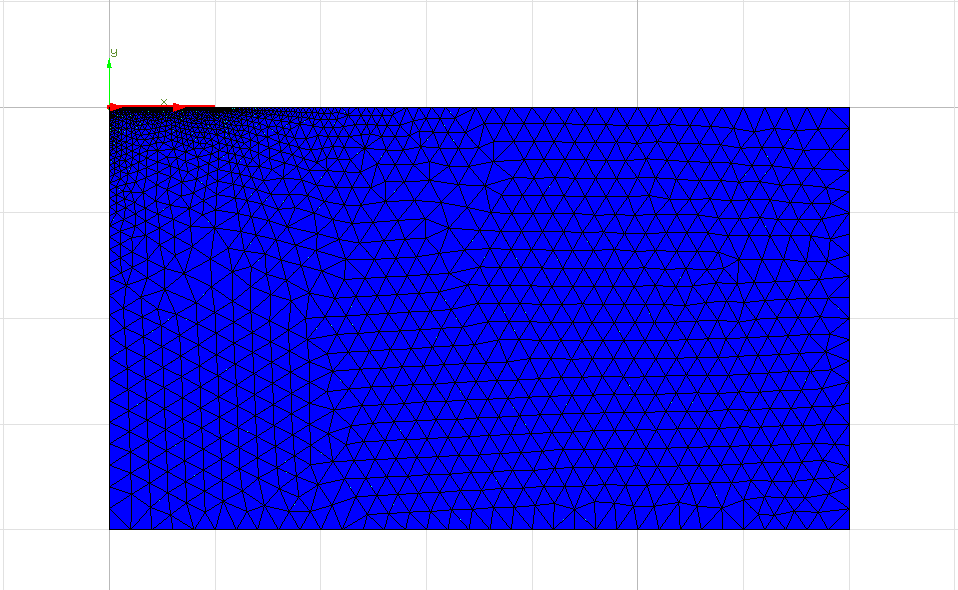
\includegraphics[width=0.50\textwidth]{figures/mesh_rigid_footing_elastic_soil.png}
	\caption{Geometry and mesh of model}
	\label{fig:rigid_footing__geometry_bm_3}
\end{figure}

\section{Material}

In this benchmark, the soil is modelled with linear elastic drained elements. The applied Youngs Modulus, $E = 1333 \space kN/m^{2}$; the applied Poisson ratio, $nu' = 0.333$.




\section{Meshing}

The mesh is generated using 6-node triangular elements. Along the footing, a mesh size is chosen of 0.015 m, within the rest of the geometry, a mesh size of 0.2 m is chosen.

\section{Results}


\begin{equation}\label{eq:reaction_force_analytical}
F = \frac{2u(1+\nu')G}{\delta} = 15.15
%u = \frac{F\delta}{2(1+\nu')G} 
\end{equation}

Since the problem is symmetric, the reaction force to compare is half the analytically calculated reaction force, i.e. $F=7.57$. 


\begin{table}[H]
	\caption{Results of reaction force for benchmark 3 with the application of a settlement }
	\label{tab:Resultsbm3}
	\centering
	\begin{tabular}{|c|c|c|c|}
		\hline
		Kratos & Plaxis 2D &Benchmark & Error\\ \hline
		[mm] & [mm] & [mm] & [\%] \\ \hline  
		$7.39$ & $7.36$ & $7.57$ & $2.43$ \\ \hline
	\end{tabular}
\end{table}


In \autoref{fig:rigid_footing_bm_3}  it is shown how the vertical stress develops underneath the rigid footing, results are shown following a Plaxis calculation, a Kratos-Geomechanics calculation and an analytical calculation. The results following the Plaxis calculation and the Kratos-Geomechanics calculation are effectively equal, both these results are in good accordance with the analytical results.

\begin{figure}[h]
	\centering
	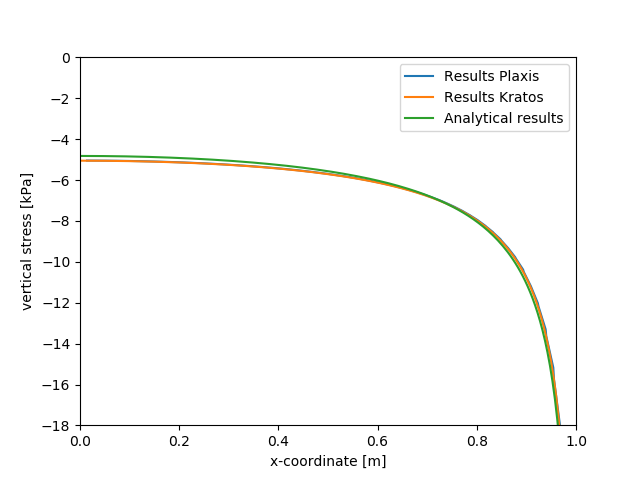
\includegraphics[width=0.50\textwidth]{figures/vertical_stress_rigid_footing_elastic_soil.png}
	\caption{Vertical stress underneath rigid footing benchmark 3}
	\label{fig:rigid_footing_bm_3}
\end{figure}


\chapter{Benchmark 4: 1D consolidation on elastic soil}
In this benchmark 1D consolidation is tested on linear elastic soil, using Kratos-Geomechanics. This benchmark includes multiple stages and a time dependent calculation.

\section{Geometry}

This benchmark is tested on a soil profile with a height of 1.0 m and a width of 0.1 m. See figure @@. The side and bottom boundaries are impermeable. At the top boundary, a 0 pore pressure condition and a line-load of 1kN/m are applied. 

@@ add figure @@

\section{Materials}
The soil is modelled with linear elastic undrained elements. The applied Youngs modulus, $E=1000\space kN/m^{2}$; the applied Poisson's ratio, $\nu'=0.0$ and the applied permeability in x- and y-direction, $k=0.001 \space m/day$.

\section{Meshing}
The mesh is generated using 6-node triangular elements with a size of 0.05 m.  




\section{Calculation}

The first phase is calculated as \textit{Soil undrained}, the following phases are calculated as \textit{Soil two phase}. All phases are calculated using the Quasi-Static solution type. The 0 pore pressure boundary condition is activated from phase 2 and onwards. In total, 11 phases are calculated at: [0.0 0.1, 0.2, 0.5, 1.0, 2.0, 5.0, 10.0, 20.0, 50.0, 100.0] days.



\begin{figure}[h]
	\centering
	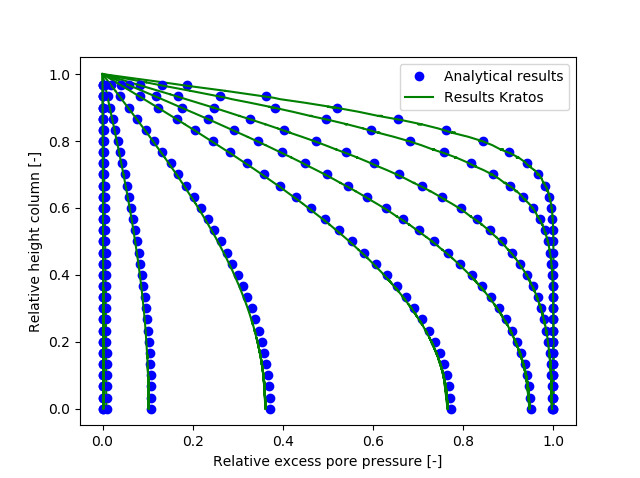
\includegraphics[width=0.50\textwidth]{figures/1d_consolidation_result.png}
	\caption{Relative excess pore pressure versus relative height on different time steps}
	\label{fig:1d_consolidation_bm_4}
\end{figure}


\section{Results}
Relative excess pore pressure can be determined analytically as a function of time and depth, as shown in the following formula [@@ref@@].

\begin{equation}\label{eq:relative_excess_pore_pressure_analytical}
\frac{p}{p_{0}} = \frac{3}{\pi}\sum_{j=1}^{\inf}\frac{(-1)^{j-1}}{2j-1}\cos[(2j-1)\frac{\pi}{2}\frac{y}{h}]\exp[-(2j-1)^{2}\frac{\pi^{2}}{4}\frac{c_{v}t}{h^{2}}]
%u = \frac{F\delta}{2(1+\nu')G} 
\end{equation}





\nonumchapter{Bibliography}
\bibliography{references/kratos_references}
\end{document}
